\chapter{Method}
\label{chap:method}
In comparison to the previous conducted studies presented in Chapter \ref{chap:related_work}, this thesis desires to bridge the research gap between emotion and personality detection and understand how personality traits can be linked to the emotions applicants express in AVIs. In order to achieve this, COGMEN is used to recognize emotions expressed in videos. A dataset is collected involving an experiment where participants answer an AVI. Applicants also answer a personality test that is used to validate the proposed personality likelihood model. 

\section{Overall description}
\label{sec:overall_description}
Figure \ref{fig:research_method} depicts the overall architecture of the research method. It consists of four parts marked in dotted squares in the figure. The first part entails investigating which benchmark dataset that is most appropriate for retrieving emotions from AVIs (Section \ref{sec:datasets}). The datasets are tested on state-of-the-art MSA model COGMEN for performance evaluation. In the second phase, a pipeline for feature extraction is developed (Section \ref{sec:feature_extraction}). A method for predicting personality out of emotions expressed in a video is established in the third part (Section \ref{sec:personality_prediction_approach}). The basis of this likelihood model are found in previous selected emotion-to-personality studies. Lastly, the fourth part is the data acquisition stage (Section \ref{sec:data_aqusition}). Participants are invited to pursue a video interview answering four interview questions. In addition, they conduct a personality test as this is used to validate the predicted results.  
\newpage
\begin{figure}[h]
  \centering
  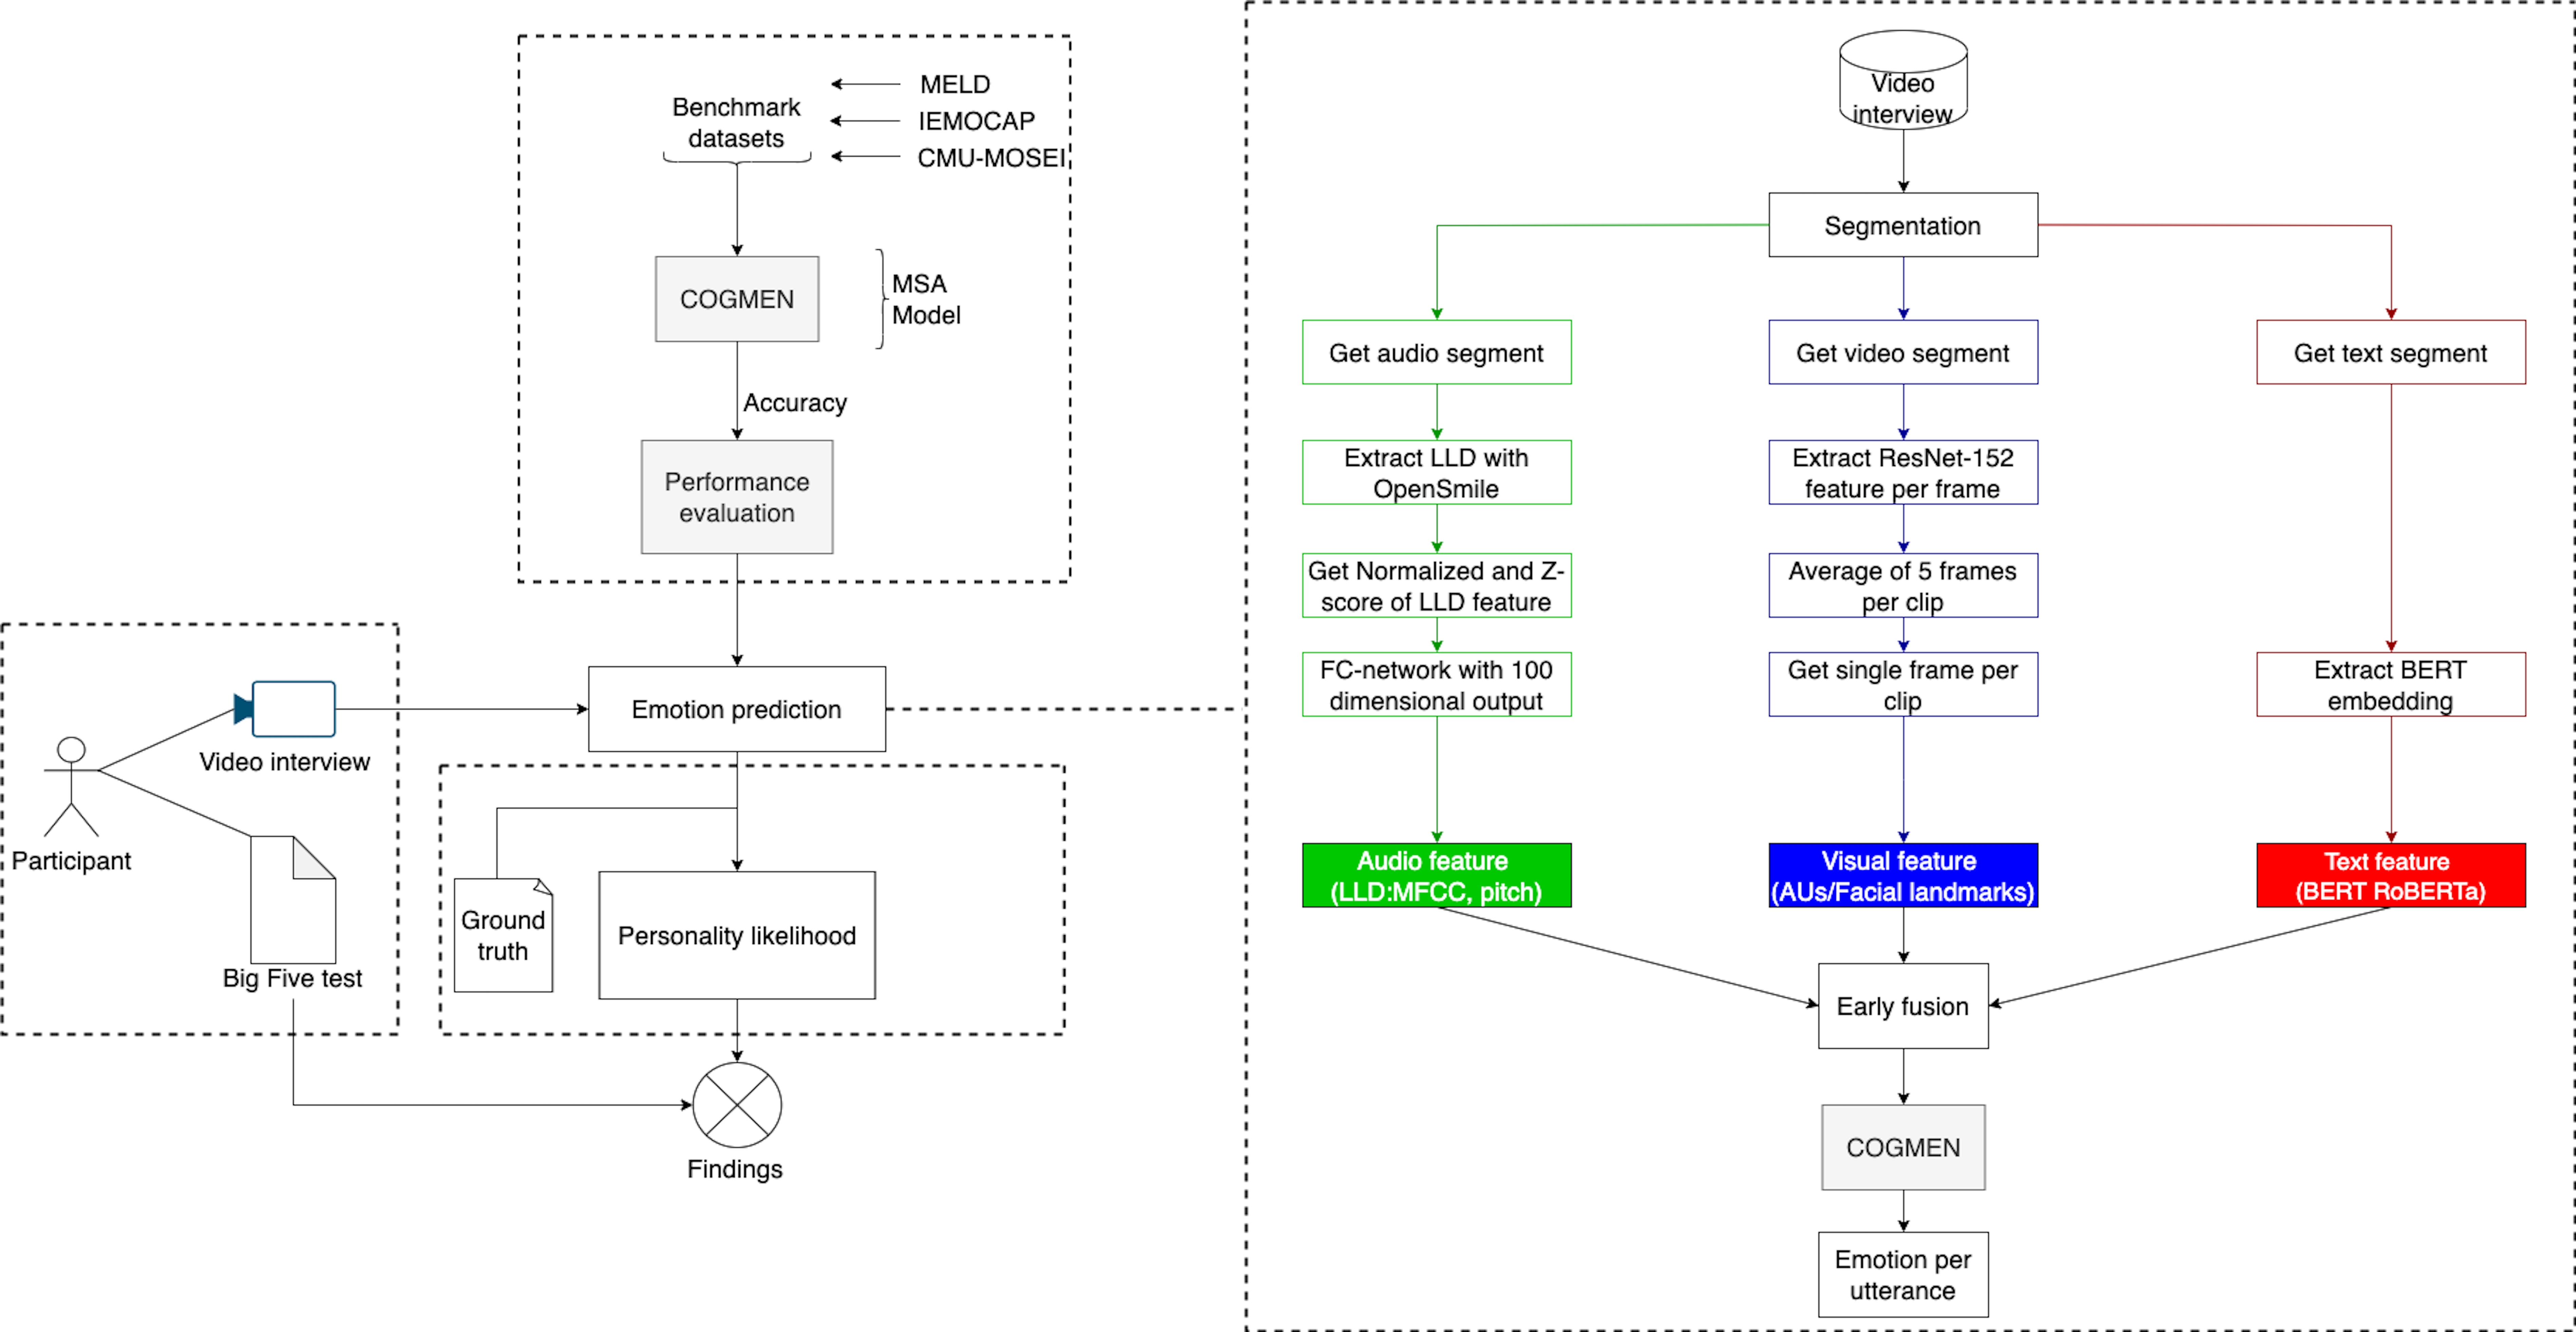
\includegraphics[width=\textwidth]{figures/new_process.png}
  \caption{Architecture of the research method.}
  \label{fig:research_method}
\end{figure}

\section{Datasets}
\label{sec:datasets}
Throughout the years, several benchmark datasets have emerged and enabled fast progress in the MSA research area \cite{COGMEN_joshi-etal-2022-cogmen}.  Table \ref{tab:datasets} lists the datasets used in this study. \textit{Modalities} denotes the different modalities of A(coustic), V(isual), and T(ext) \cite{HP_RPP} \cite{HP_Advanced}. \textit{\#v} indicates the total number of video segments and \#s designates the total number of speakers. \textit{Sent} denotes whether or not the dataset contains sentiment annotations and \textit{Emo} denotes whether or not the dataset contains emotion annotations. \textit{TL} is the total length of the dataset. 
%
\begin{table}[h]
\caption{Benchmark MSA datasets used in the thesis.}
\centering
\resizebox{\textwidth}{!}{%
\begin{tabular}{|l|l|l|l|l|l|l|l|l|}
\hline
\multicolumn{1}{|c|}{\textbf{Name}} & \multicolumn{1}{c|}{\textbf{Year}} & \multicolumn{1}{c|}{\textbf{Modalities}} & \multicolumn{1}{c|}{\textbf{\#V}} & \multicolumn{1}{c|}{\textbf{\#S}} & \multicolumn{1}{c|}{\textbf{Sent}} & \multicolumn{1}{c|}{\textbf{Emo}} & \multicolumn{1}{c|}{\textbf{Lang}} & \multicolumn{1}{c|}{\textbf{TL (hh:mm:ss)}} \\ \hline
 MELD \cite{meld_dataset} & 2019 & A + V + T  & 13 000 & Multi speaker & Yes & Yes & English & -  \\ \hline
 CMU-MOSEI \cite{cmu-mosei_zadeh2018multimodal} & 2018  & A + V + T  & 23 500 & 1000 & Yes & Yes & English & 65:53:36   \\ \hline
 IEMOCAP \cite{iemocap_dataset} & 2008 & A + V + T  & 10 000 & 10 & No & Yes & English & 11:28:12  \\ \hline
\end{tabular}
}
\label{tab:datasets}
\end{table}

\subsection{MELD dataset}
Multimodal EmotionLines Dataset (MELD) is an emotion recognition dataset for multi-party conversations \cite{meld_dataset} \cite{HP_Advanced}. It is an extension of the EmotionLines Dataset. The EmotionLines only contains textual data, but MELD includes their corresponding visual and audio counterparts. MELD contains approximately 1400 dialogues and 13,000 utterances from the popular sitcom called Friends. Each utterance is a part of a dialogue and 42\% of the utterances are shorter than five words. The dataset is annotated with emotion and sentiment labels. Each speech in a dialogue is labeled with one of the following emotions: Anger, Disgust, Sadness, Joy, Neutral, Surprise, and Fear. In addition, all utterances are assigned a sentiment (positive, negative, neutral). 

\subsection{CMU-MOSEI dataset}
CMU Multimodal Opinion Sentiment and Emotion Intensity (CMU-MOSEI) is the largest dataset of sentence level sentiment analysis and emotion recognition in online videos \cite{MSA_review2_GANDHI2023424} \cite{cmu-mosei_zadeh2018multimodal} \cite{HP_Advanced}. Videos are collected from YouTube, and the total length of the dataset is over 65 hours. Out of 3228 videos, there are 23,453 annotated data points from 1000 distinct speakers covering 250 subjects. Each video segment contains manual transcription aligned with audio to phoneme level. The sentences are assigned sentiment annotations ranging from [-3, 3] and emotions labels (i.e., Happy, Sad, Angry, Fear, Disgust, Surprise). CMU-MOSEI includes various topics where the most frequent topics are reviews, debate, and consulting. 

\subsection{IEMOCAP dataset}
Interactive emotional dyadic motion capture database (IEMOCAP) is a widely used dataset for performing emotion recognition tasks \cite{iemocap_dataset} \cite{HP_Advanced}. It consists of 10,000 segments of audiovisual data, including speech, facial expression and hand gestures, and text in dyadic conversations. IEMOCAP is captured from 10 different actors that perform fictitious conversations to elicit different emotions including Happy, Sad, Neutral, Angry, Excited, and Frustrated. In addition, this dataset uses continuous attribute based annotations such as activation, valence and dominance. Both these annotations methods are assigned each utterance in a conversation. The total length of IEMOCAP is just under 12 hours. \\

Table \ref{tab:datasets_splitting} shows data splitting for each data set into train, validation and test. For hyperparameter tuning, the Bayesian optimizer was used. Table \ref{tab:datasets_hyperparameter} illustrates the hyperparameter setting on the datasets utilized to train COGMEN. 
%
\begin{table}[h]
\caption{Data splitting.}
\centering
\resizebox{3.5in}{!}{%
\begin{tabular}{|l|l|l|l|l|}
\hline
\multicolumn{1}{|c|}{\textbf{Name}} & \multicolumn{1}{c|}{\textbf{Train}} & \multicolumn{1}{c|}{\textbf{Validation}} & \multicolumn{1}{c|}{\textbf{Test}} & \multicolumn{1}{c|}{\textbf{All}} \\ \hline
MELD & 9989 & 1108 & 2610 & 13707 \\ \hline
CMU-MOSEI & 16326 & 1871 & 4659 & 22856 \\ \hline
IEMOCAP & 5354 & 528 & 1650 & 7532\\ \hline
\end{tabular}
}
\label{tab:datasets_splitting}
\end{table}
%
%
\begin{table}[h]
\caption{Hyperparameter settings for each dataset. \textit{ILR} denotes initial learning rate.}
\centering
\resizebox{4.0in}{!}{%
\begin{tabular}{|l|l|l|l|l|}
\hline
\multicolumn{1}{|c|}{\textbf{Name}} & \multicolumn{1}{c|}{\textbf{Dropout}} & \multicolumn{1}{c|}{\textbf{GNNHead}} & \multicolumn{1}{c|}{\textbf{SeqContext}} & \multicolumn{1}{c|}{\textbf{ILR}} \\ \hline
MELD & 0.105 & 7 & 4 & 1.3e-4 \\ \hline
CMU-MOSEI & 0.340 & 2 & 1 & 1.1e-3 \\ \hline
IEMOCAP & 0.1 & 6 & 3 & 1.0e-4\\ \hline
\end{tabular}
}
\label{tab:datasets_hyperparameter}
\end{table}
%
Feature extraction for MELD and IEMOCAP is performed with the established feature extraction pipeline. When it comes to CMU-MOSEI features, the author tried to follow the method presented in \cite{cmu-mosei_zadeh2018multimodal}. However, extracting visual features was impossible, since FaceNet 2.0, a facial expression extraction tool, is not open source. Therefore, the authors of COGMEN were contacted in order to receive acoustic, visual, and textual features for CMU-MOSEI in Multi-label classification setting. Results form the performance evaluation is presented in Section \ref{sec:performance_evaluation}.

\subsection{Evaluation metrics}
To evaluate COGMEN on the various datasets, widely used evaluation metrics are adopted such as:
%
\begin{equation*}
    Accuracy = \frac{TP+TN}{TP+TN+FP+FN},\tag{15}
\end{equation*}
%
\begin{equation*}
    F1 = \frac{2 \cdot precision \cdot recall}{precision + recall},\tag{16}
\end{equation*}
%
Where \textit{TP}, \textit{TN}, \textit{FP}, \textit{FN} designate the number of true positives, true negatives, false positives, and false negatives, respectively \cite{HP_Advanced}. On all three datasets, we use the weighted F1 score for emotion classification. 

\section{Feature extraction pipeline}
\label{sec:feature_extraction}
Today's feature extraction methods are dominant as per problem requirement. Therefore, it is necessary to create processes that automatically extracts features from multimodal data. As feature extraction is an important process of multimodal fusion, a feature extraction pipeline is developed for emotion recognition in COGMEN. This process is depicted in the right side of Figure \ref{fig:research_method}. 

\subsection{Data preparation}
Data preparation is essential before extracting meaningful information from three modalities. A video consists of the following modalities: $a$(acoustic), $v$(visual), and $t$(textual) which are 2D tensors denoted by $M_{a} \in R^{T_{a} \times d_{a}}$, $M_{v} \in R^{T_{v} \times d_{v}}$, $M_{t} \in R^{T_{t} \times d_{t}}$, where $T_{m}$ and $d_{m}$ represent sequence length and feature vector size of modality $m$. The raw video is divided into segments (i.e. utterances). For a given raw video $v$, it is separated into $U_{m} = [u_{1}, u_{2}, u_{3}, ..., u_{n}]$ utterances where $m\in\{a, v, t\}$. For MELD and IEMOCAP, utterances are divided by change of speakers. However, in the AVI dataset(presented in Section \ref{sec:data_aqusition}), only one speaker is present. Therefore, each utterance is separated by speech pauses. In addition, the candidates are asked to say each question out loud before responding, making the segmentation process more effective. 

\subsection{Acoustic features}
Acoustic features are extracted with 30 Hz frame-rate and a sliding window of 100 ms using OpenSMILE toolkit \cite{opensmile}. These features consists of low-level descriptors (LLDs) including voice intensity and pitch with their corresponding statistics. One challenge with audio feature extraction is to identify segments with and without voice. To cope with this issue, a Z-score standardization was employed to the LLDs for voice normalization as done in \cite{z-score-8215597}. Further, the normalized features are fed to a CNN model with a fully connected layer containing 100 nodes resulting in the 100-dimensional audio feature vector $[u_i^{(a)}]\in R^{d_{a}}$. 

\subsection{Text features}
For text features, the Google Cloud Speech API \footnote{\url{https://cloud.google.com/speech-to-text}} is used to create text transcripts for each utterance. Transformer-based pre-trained BERT is utilized as the text encoder \cite{BERT-reimers2019sentence}. The raw sentence $S = (w_{1}, w_{2}, w_{3}, ..., w_{n})$ composed of word indices is first concatenated with two special tokens - [CLS] at the head an [SEP] at the tail an then fed into the encoder to generate contextualized word embeddings,  resulting in the high-dimensional text feature vector $[u_i^{(t)}]\in R^{d_{t}}$. 

\subsection{Visual features}
The visual feature extraction consists of several steps. First, the each video segment were converted into a series of frames. Then, the Multi-task Cascaded Convolutional Network (MTCNN) \cite{MTCNN-9239720} is used to detect the faces in each frame. MTCNN is used because is reported to be accurate and robust. The MTCNN is also able to detect faces in various lighting settings, different distances from the camera, and even with strong head rotations. Furthermore, a Residual Network (ResNet) with 152 layers is utilized to extract feature vector with size 512. One frame from each utterance is computed by the average of 5 frames for each utterance. The feature can be represented as $[u_i^{(v)}]\in R^{d_{v}}$. \\

The acoustic, visual, and textual features are concatenated using early fusion, as this fusion process provides the best performance of COGMEN \cite{COGMEN_joshi-etal-2022-cogmen}. The feature vector for an utterance $u_{i}$ with the aforementioned input features from three modalities is:
%
\begin{equation*}
    x_{i}^{(atv)} = [u_{i}^{(a)} \oplus u_{i}^{(t)} \oplus u_{i}^{(v)}] \in R^{d},\tag{17}
\end{equation*}
%
where $d = d_{a} + d_{t} + d_{v}$. 

\section{Personality prediction approach}
\label{sec:personality_prediction_approach}
Using MSA for personality prediction is something new. To the best of my knowledge, there exist no studies that aim to predict human attributes based on emotions expressed in AVIs. Additionally, there do not exist any multimodal datasets with labeled emotions and corresponding personality traits. Therefore, it is difficult to create DL models that perform both emotion recognition and personality prediction. Another problem regarding the two tasks, is that each distinct emotion are linked to several personality traits. The proposed approach takes the emotion distribution in order to forecast the likelihood of the most dominant traits. Because the Big Five describes a continuum of traits, each person is not associated with all traits. Therefore, the model predicts the three strongest traits in an interviewee. The basis of the likelihood model are from the emotions-to-personality relationship studies \cite{personality-and-emotion-revelle2009personality},  \cite{extraversion1-komulainen2014effect}, \cite{personality_emotions_link}, \cite{personality1-deyoung2007between}, \cite{personality2-9210819}, and \cite{emotion_personalty_correlation_Zhao2018}. As shown in Figure \ref{fig:emotion_traits_link}, each personality trait has the following emotion relationship:
%
\begin{itemize}
    \item Openness is associated with a mix of positive and negative emotions. The expression of mixed emotions tend to happen through emotional occasions such as graduation day or discussing accomplishments. \\
    \item Conscientiousness is linked to neutral emotions. Research show that people with high scores in conscientiousness experience lower level of emotions in general and it is more difficult for them to elicit these emotions. \\
    \item Extraversion is related to a higher positive effect (i.e. happiness and excited). \\
    \item Agreeableness is connected to positive emotions. In addition, this trait is correlated with conscientiousness where these two traits are in line with each other. \\
    \item Neuroticism is solely associated with negative emotions (i.e. anger, frustration, and sadness).
\end{itemize}
\newpage
\begin{figure}[h]
  \centering
  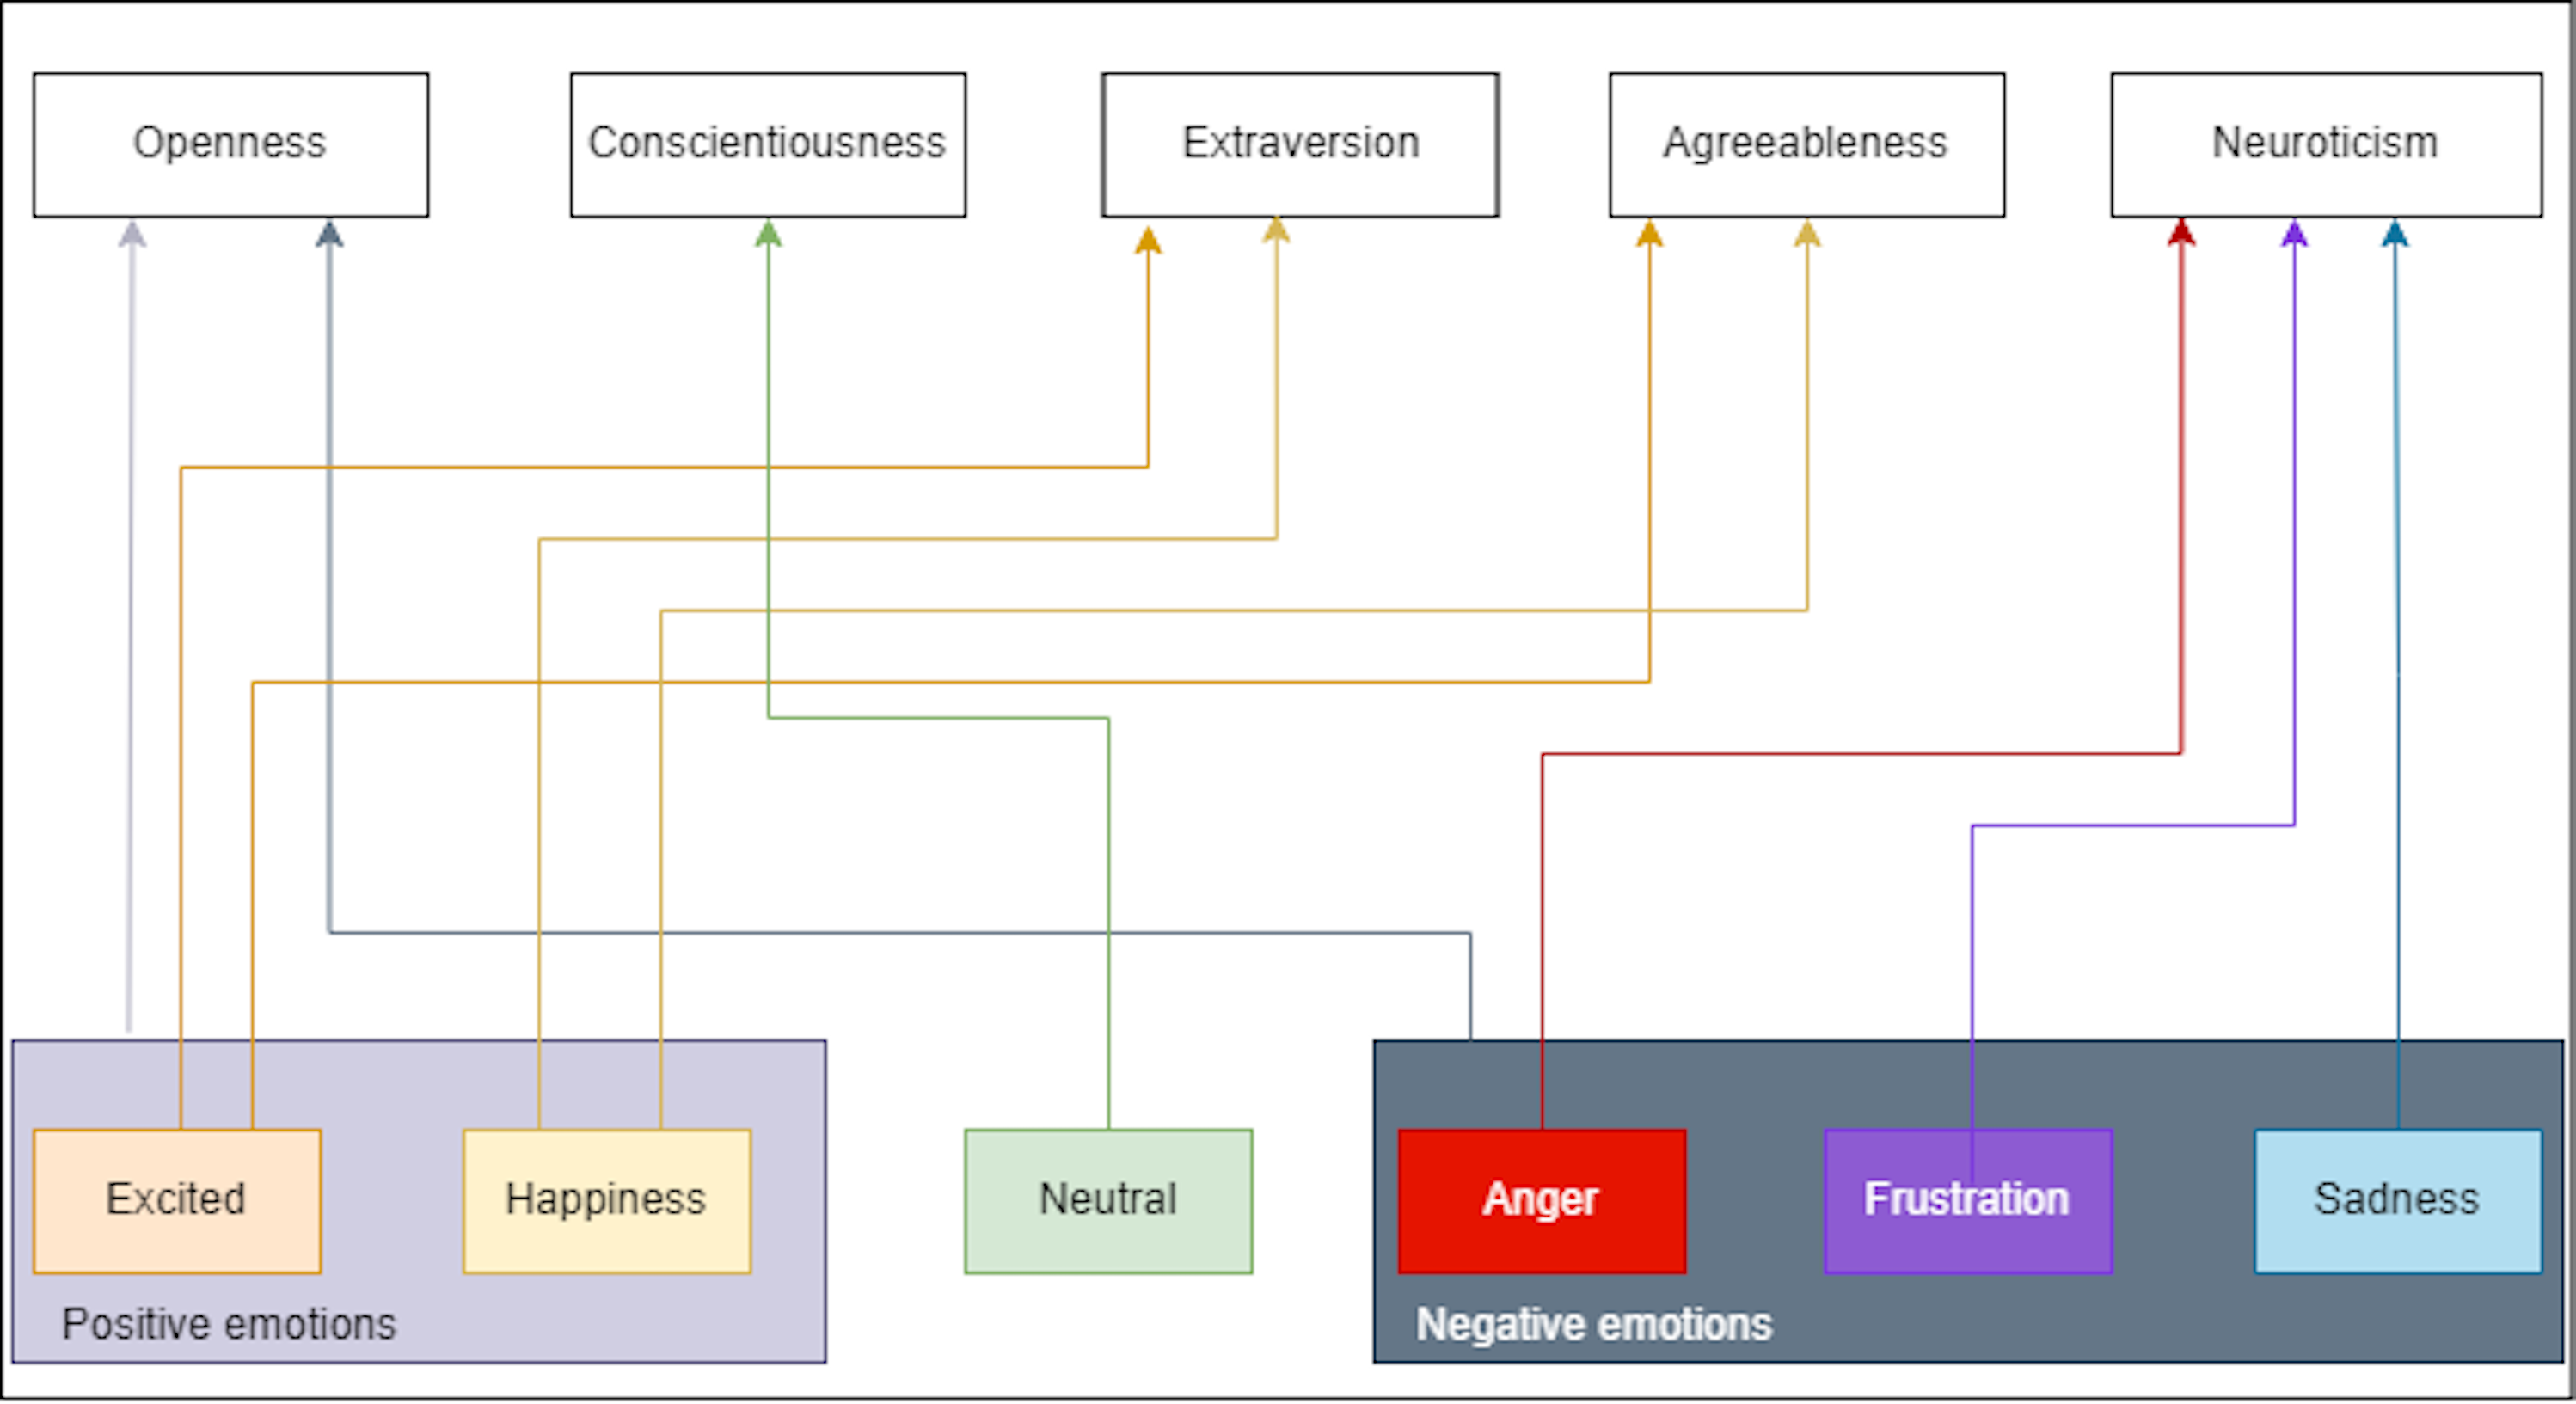
\includegraphics[width=\textwidth]{figures/emotion_traits_link.png}
  \caption{Relationship between emotions and personality traits.}
  \label{fig:emotion_traits_link}
\end{figure}

\subsection{Example of predicting personality}
To provide examples, the procedure of predicting the three strongest personality traits of an applicant is presented in this section. The emotion distribution of sample 1 is illustrated in Figure \ref{fig:emotion_personality1}. The emotions are normalized to 0 - 1 by the sum of an emotion per video over the total number of emotions for a given video. As can be seen from the distribution, there is a mix of positive and negative emotions. Accordingly, there is a high likelihood that the candidate's highest scoring trait is openness. Further, the applicant express a high degree of negative emotions, where sadness is recognized in 35 \% of the interview. The suggestion is therefore that the person has a high score in neuroticism. Lastly, the candidate showcases both excited and happy emotion. Because there is a low chance that the person is conscientious, extraversion is predicted higher than agreeableness. To summarize, person 1 is predicted as:
%
\begin{equation*}
    [Openness, Neuroticism, Extraversion],
\end{equation*}
%
presented in a descending order with the strongest trait first.
%
\begin{figure}[h]
  \centering
  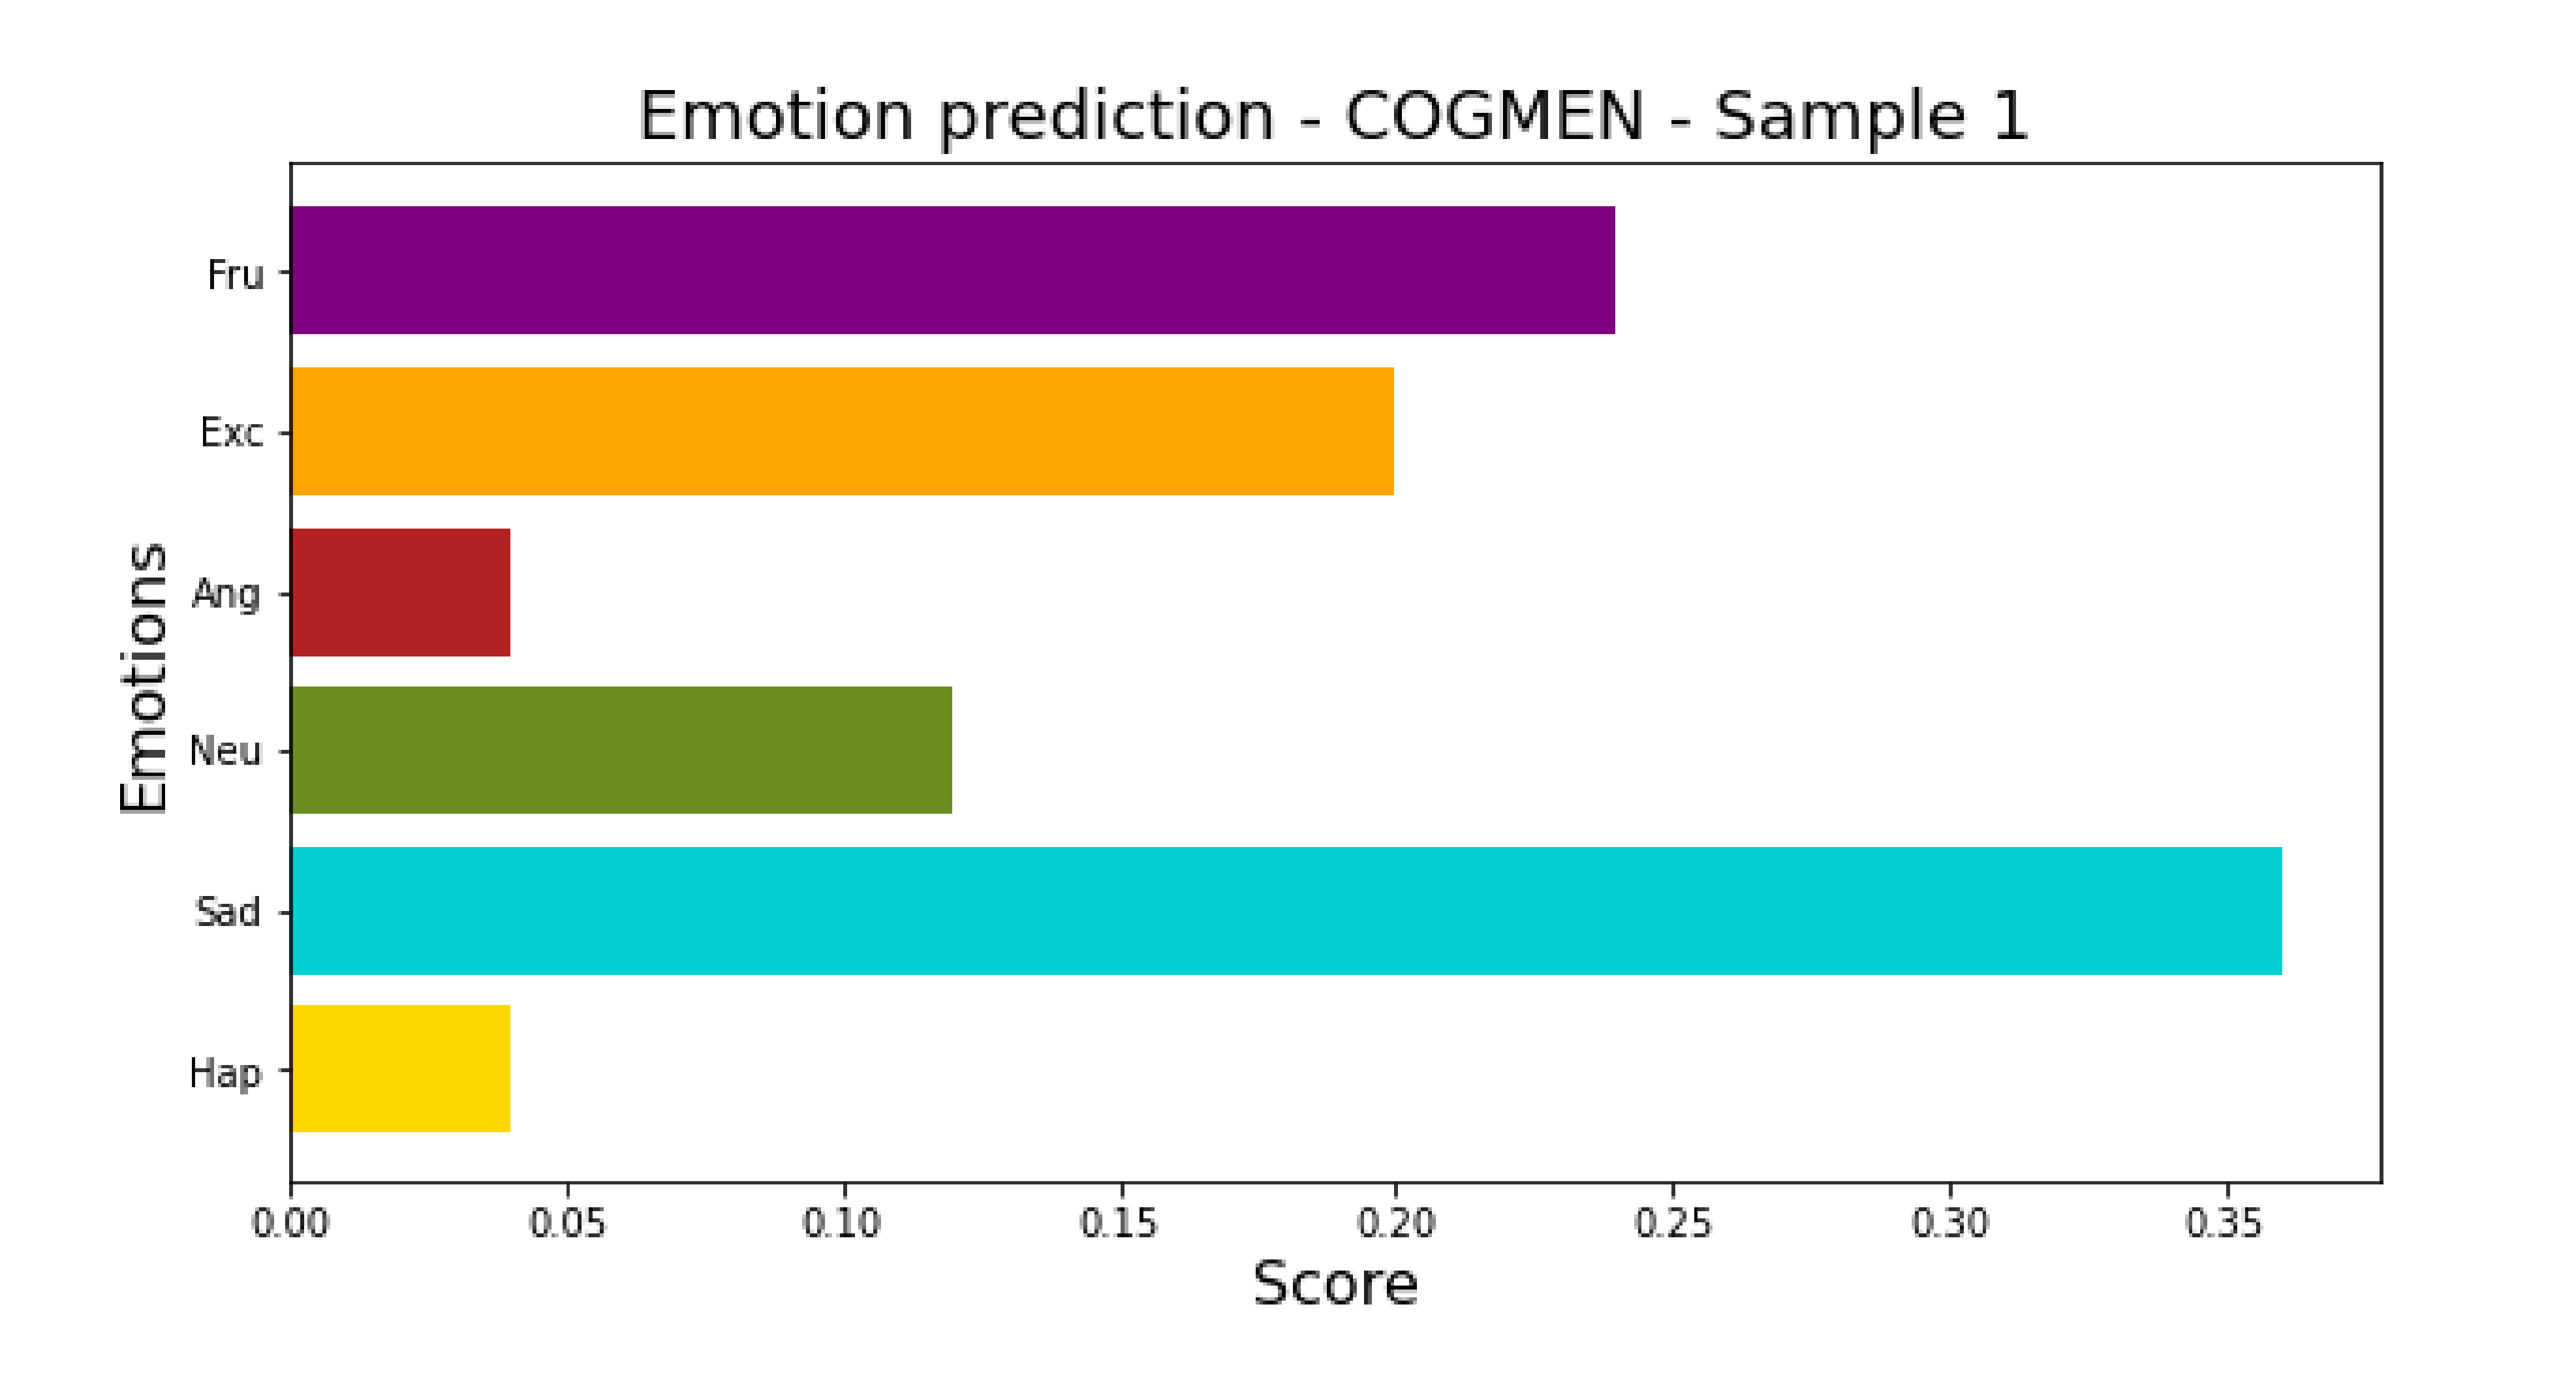
\includegraphics[width=\textwidth]{figures/emotion_distribution_sample1.png}
  \caption{Emotion distribution of interviewee 1.}
  \label{fig:emotion_personality1}
\end{figure}
%
\newline
\indent Another sample is depicted in Figure \ref{fig:emotion_personality4}. The participant has a different emotion distribution than the one in sample 1. As can be seen from the figure, the majority of expressed emotions is neutral. Therefore, there is a large likelihood that the strongest trait in applicant 4 is conscientiousness. Moreover, conscientiousness i correlated with agreeableness. Consequently, agreeableness is predicted as the second trait. Finally, the rest of the distributions illustrates a mix of positive and negative affect resulting in the third personality trait being openness. To conclude, participant 4 has the following traits:
%
\begin{equation*}
    [Conscientiousness, Agreeableness, Openness]
\end{equation*}
%
\newpage
%
\begin{figure}[h!]
  \centering
  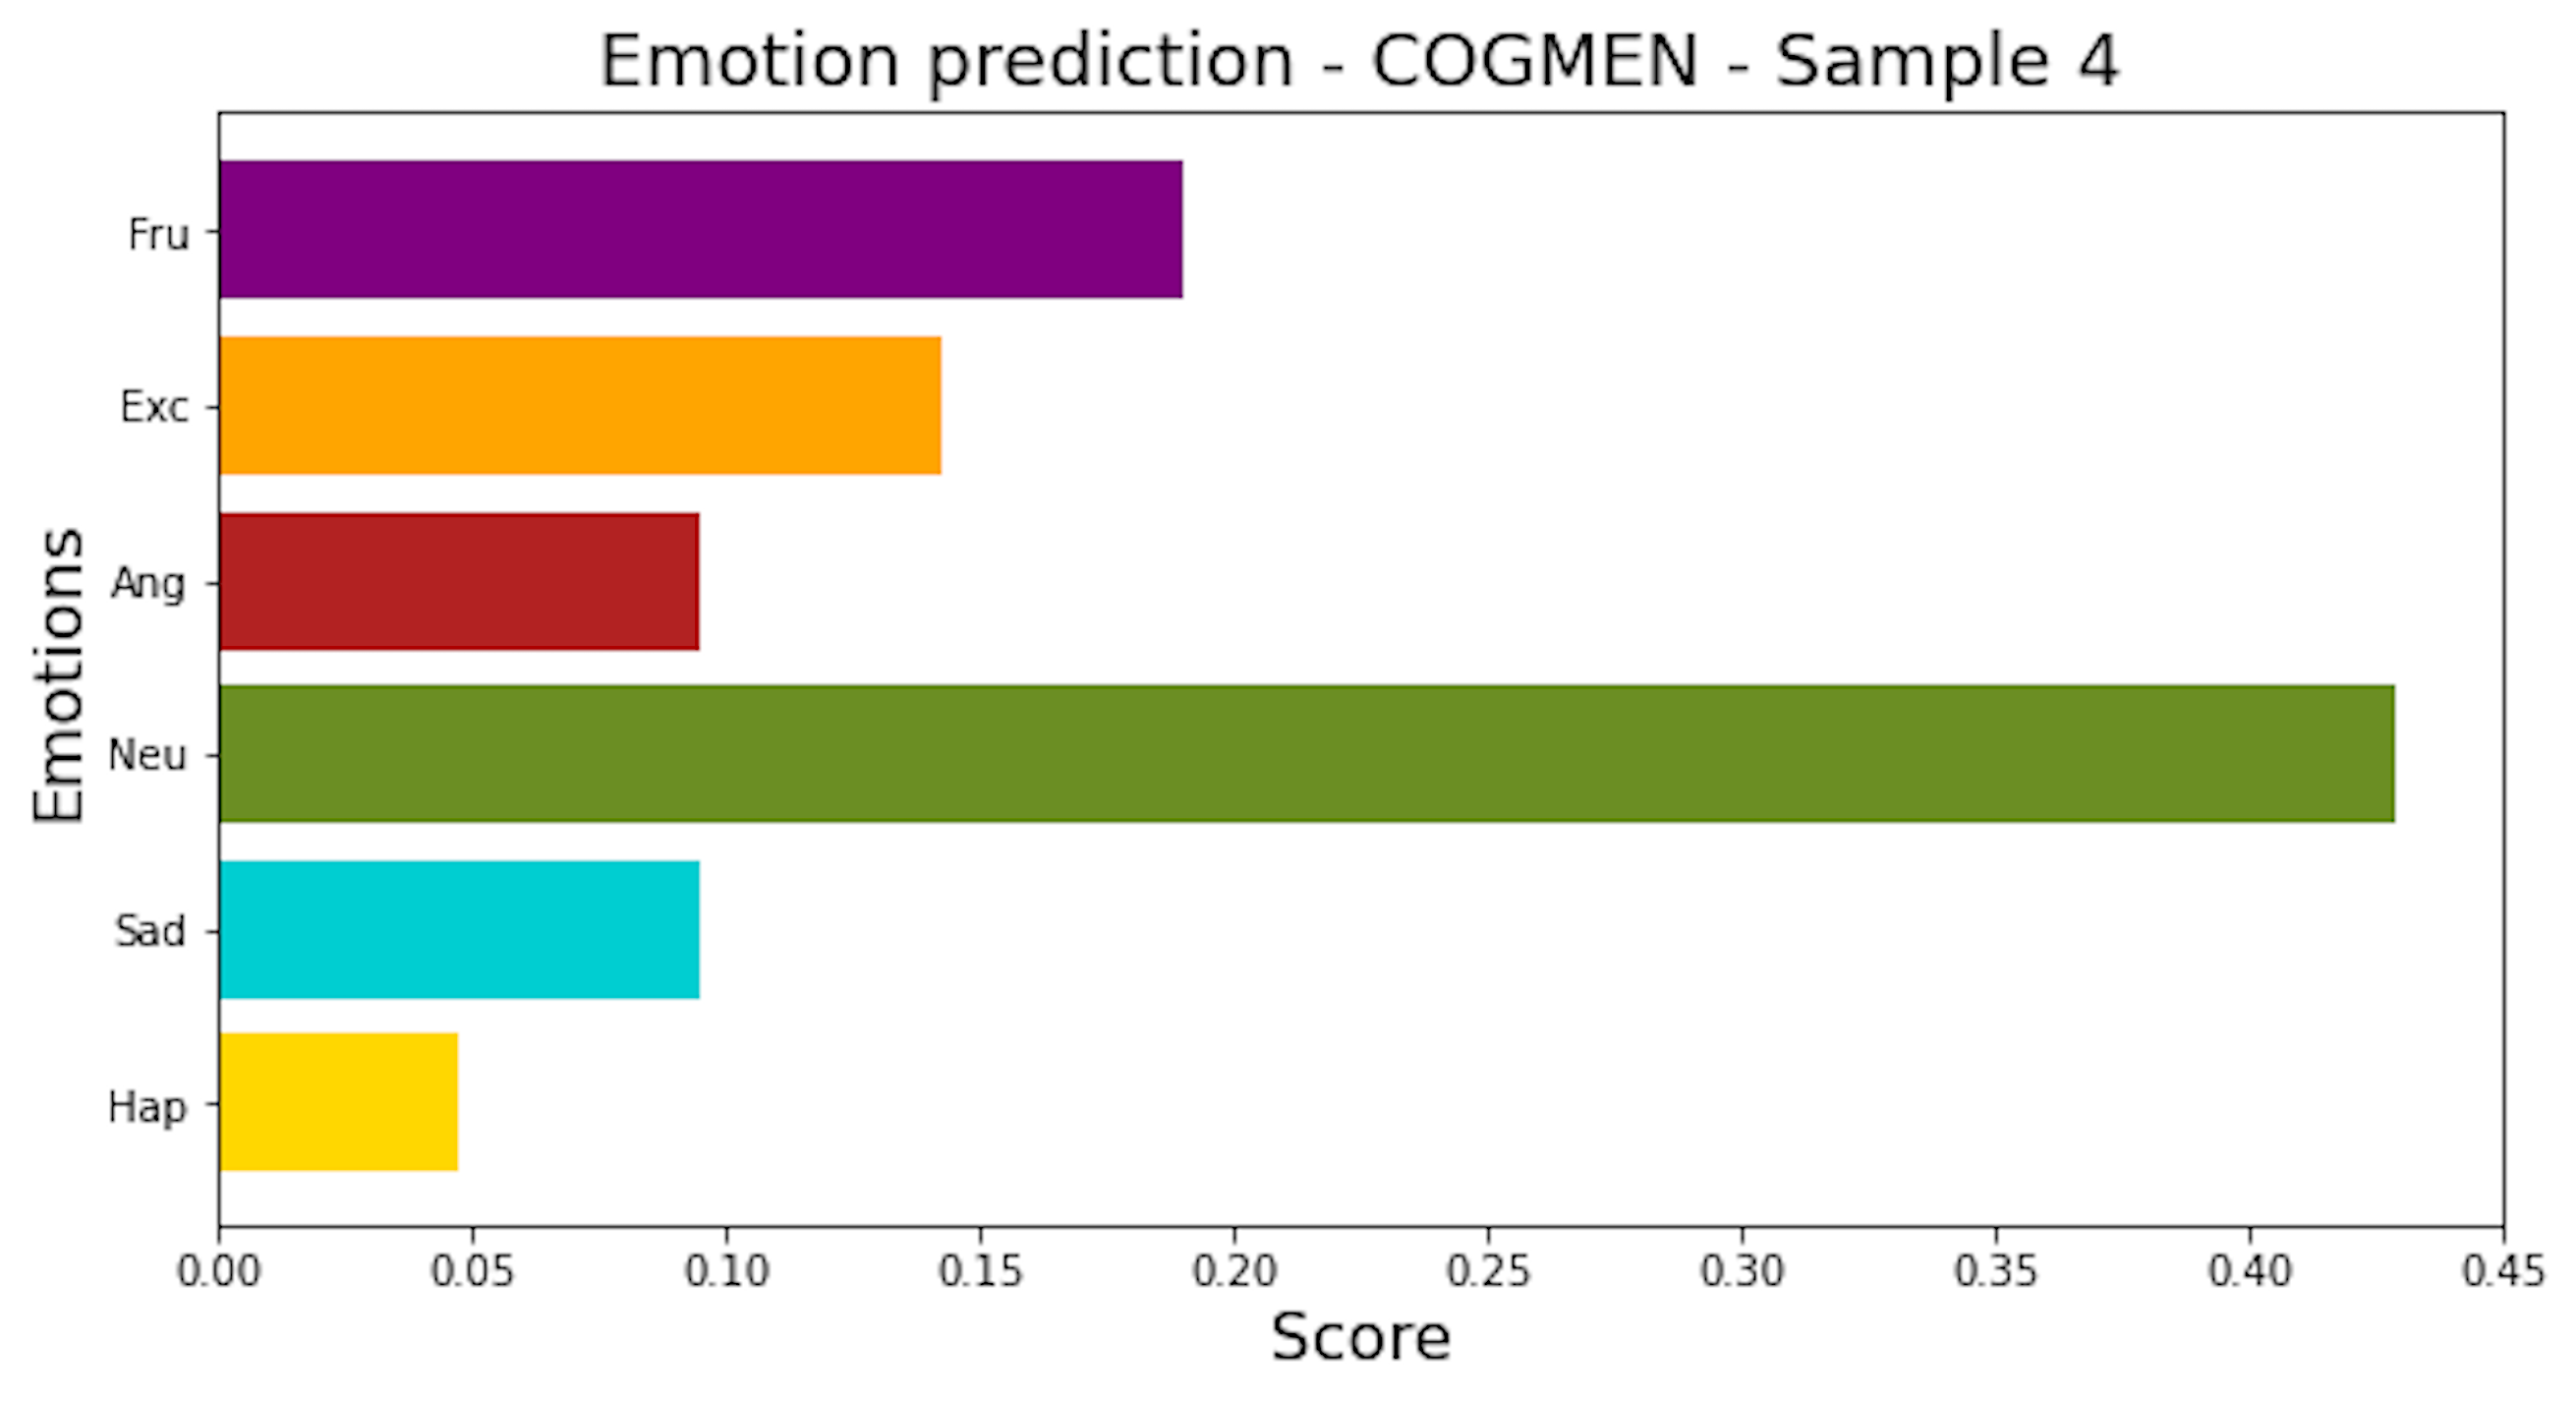
\includegraphics[width=\textwidth]{figures/emotion_distribution_sample4.png}
  \caption{Emotion distribution of interviewee 4.}
  \label{fig:emotion_personality4}
\end{figure}
%

\section{Data acquisition}
\label{sec:data_aqusition}
The data acquisition consists of two parts: The first part is an AVI where participants record themselves answering interview questions. The second part entails answering a personality questionnaire based on the Big Five model. These two parts are separate tasks, meaning that the interview and personality test can be taken in any order preferred by the entrant. 

\subsection{Participants}
A total of seven candidates participated in the study. All are men from Norway. Another common denominator is that they are in an informatics study program. The participants are also at the end of their studies and in an job seeking position. 

\subsubsection{Ethical and legal considerations}
In this study, personal data (i.e. AVIs) is collected and thus several ethical and legal aspects should be considered. Before starting collecting interviews, a notification form about the data acquisition was sent to Sikt/NSD for evaluation if the process complied with the General Data Protection Regulation (GDPR). Each participant was provided a participation form as shown in Appendix \ref{apx:participation_form} to give information about the study as well as obtaining consent. The privacy and confidentiality of the interviewees was at the forefront at all times. Data about the participants were de-identified and assigned unique identifiers.  

\subsection{Video interview}
\label{sec:video_interview}
In the video interview, it is desired to simulate how companies conduct their AVIs in real life. Therefore, the AVI design is thoroughly deliberated before participants pursue the experiment. Table \ref{tab:our-AVI-design-features} shows the AVI design used in the experiment. Experiment introductions and interview questions are presented in written format which makes it easy to provide the same information to all participants. The experiment instructions are found in Appendix \ref{apx:video_recording_instructions}. This information sharing reduces media richness, meaning that observers will lack the perception of social presence. However, providing rich media features that seamlessly mimic a live interview is challenging when an AVI platform is not used. There is no question timers in the interview, but it is implied that each participant uses a reasonable amount of time to understand the questions. \\

When it comes to the response preparation time, observers could view the questions right before the recording happened. The reason for this choice, is because people tend to express more emotions in the behavioral cues such as visual and audio if the preparation time is small \cite{video-interview1-LUKACIK2022100789}. For example, when a person have to improvise a question answer, they become more expressive in their face showing gestures like frowns and smiles, and it affects their audio cues where they take pauses, stutter, or their voices shake. In addition, the little time to prepare an answer automatically provides an overview of the candidates' communication skills. Nevertheless, there are two major disadvantages with this response formatting feature which can lead to negative applicant outcomes. First, this setting is associated with a perception of low fairness meaning that the participants become unmotivated to complete the interview. Second, people with poorer communication skills will give responses of mediocre quality. As the text is the most important modality in MSA, the performance of MSA models will be negatively affected. Consequently, it is essential that each observer produces good responses to the interview questions. To mitigate the aforementioned downsides, interviewees have the ability to re-record their responses up to three times allowing them to choose their best recorded performance for submission. There is no time cap for the candidate to complete the interview. However, it is stated that they are supposed to complete the interview in one go reducing the risk of people prepare their answers in the time between the responses. \\

The total length allowed for the candidates to answer each interview question is set to minute. Given that prior research are able to retrieve emotions and personality traits from small video clips supports this reasoning \cite{model_based_fusion6122012} \cite{video-interview4-SUMAN2022107715}. Candidates have the ability to review their responses before moving on to the next question. Additionally, the interviewees have a live recording preview windows because the impact of applicant deceptive impression management (i.e. the behaviors people use to shape how they are viewed by others) on interview performance is smaller in AVIs with video recording previews \cite{video-interview1-LUKACIK2022100789}. Lastly, the evaluation feature is based on automated assessment. The videos are used as input in MSA models and emotions are predicted as output. Utilizing automated evaluators enhances the screening process speed as well as reducing the impact of subjective bias and the adverse impact against protected groups. At one hand, the use of AI-systems to rate participants may lead to an increase in interview refusals. At the other hand, people are more positive tuned when they are informed that the AVI contain automated assessment and how the system will infer each applicant. 
%
\begin{table}[h]
    \caption{AVI design features for the experiment.}
    \centering
    \resizebox{\columnwidth}{!}{%
    \begin{tabular}{l p{9.4cm}}
     \toprule
     \multicolumn{2}{c}{\textbf{Media features}} \\ \\ 
     Video introductions & Video introductions and the set of interview questions are presented in written format. \\ \\ 
     \midrule 
     \multicolumn{2}{c}{\textbf{Response formatting features}} \\ \\ 
     Response preparation time & The candidates should view the questions right before the recording happens. \\ \\ 
     Re-recording responses & The candidates have the ability to re-record each question up to three times. \\ \\ 
     Interrupted interview completion & The candidates should pursue the recording in one go. \\ \\ 
     Length of allowed response & The total length for each response is one minute.\\ \\ 
     Video recording preview & A live recording preview window is facilitated for the participants to view themselves while recording their responses.  \\ 
     \midrule
     \multicolumn{2}{c}{\textbf{Evaluation features}} \\ \\ 
     Automated assessment & The recording are used as input in a MSA model and the output is a predicted emotion. \\ 
     \bottomrule
    \end{tabular}
    }
    \label{tab:our-AVI-design-features}
\end{table}
%
This AVI is similar to a structured live interview because each candidate is asked the same questions and evaluated based on fixed criteria. Advantages having such interview setting are the reduce of bias and an increased ability to predict future job performance \cite{increase-job-performance-mcdaniel1994validity}. Choosing the appropriate type of questions is essential in order for the participants to express their emotions when pursuing the interview. The participants were asked to answer four different questions. All questions were asked in the same order for each applicant. Following are the questions used in the AVI:
%
\begin{itemize}
    \item[] Q1: What motivates you? What are you passionate about?
    \item[] Q2: Not everyone agrees all the time. Have you had a peer, teammate or friend disagree with you? What did you do?
    \item[] Q3: Give an example of a time you have gone over and above to achieve something. Why was it important for you to achieve this?
    \item[] Q4: Sometimes things don’t always go to plan. Describe a time when you failed to meet a deadline or personal commitment. What did you do? How did that make you feel?
\end{itemize}
%
The four questions are open-ended. Open-ended interview questions provide a conducive environment for the interviewees to express their emotions by allowing them the freedom to explore and articulate their thoughts and feelings. As these questions are based on past behavior, situational judgement, and values, they encourage individuals to delve deeper into their experience and requires thoughtful reflection. This approach invites personal narratives, introspection, and emotional expression, allowing interviewees to provide richer and more nuanced responses that encompass their genuine emotional experiences \cite{personality-prediction-questions-9121971} \cite{emotions_question_johnson2020emotions}. Moreover, the questions allow the participants to elicit the whole spectrum of various emotions. For example, Q1 and Q3 are targeting positive emotions, whereas Q2 and Q4 target negative emotions. \\

The recordings were captured using the Zoom application \footnote{\url{https://zoom.us/}}. There are three reasons for using this application. First, almost every student have Zoom on their devices. In that case, the participants avoid unnecessary downloads of applications that they have to become familiar with. Second, Zoom provides a recording quality up to 1080p(1920p x 1080p) which is important for MSA to recognize visual cues. Lastly, the application is available on all devices (computer, tablet, phone, etc.). It is essential to accommodate the participants by enabling them to perform the AVI with their preferable device. The new acquired dataset is called the AVI dataset. Dataset statistics are presented in Table \ref{tab:new_dataset}. \textit{Modalities} denotes the different modalities of A(coustic), V(isual), and T(ext). \textit{\#v} indicates the total number of video segments, \textit{Lang} denotes language, and \#s designates the total number of speakers. \textit{TL} is the total length of the dataset.  
%
\begin{table}[h]
\caption{AVI dataset statistics.}
\centering
\resizebox{\columnwidth}{!}{%
\begin{tabular}{|l|l|l|l|l|l|l|l|l|}
\hline
\multicolumn{1}{|c|}{\textbf{Name}} & \multicolumn{1}{c|}{\textbf{Year}} & \multicolumn{1}{c|}{\textbf{Modalities}} & \multicolumn{1}{c|}{\textbf{\#v}} & \multicolumn{1}{c|}{\textbf{\#s}}  & \multicolumn{1}{c|}{\textbf{Lang}} & \multicolumn{1}{c|}{\textbf{TL (hh:mm:ss)}} \\ \hline
 AVI dataset & 2023 & A + V + T  & 180 & 7 & English & 00:38:34 \\ \hline
\end{tabular}
}
\label{tab:new_dataset}
\end{table}

\subsection{Big Five personality test}
A personality test is conducted for participants to assess their own personality. They answered the Big Five personality test \footnote{\url{https://bigfive-test.com/}}, an open-source personality questionnaire. Test and evaluation is gathered from the 120-item IPIP NEO-PI-R, which is favoured compared to the IPIP-NEO 300-item inventory \cite{JOHNSON201478}. The personality inventory consists of 120 statements that are rated on a 5-point scale from strongly agree to strongly disagree. Following are some example statements from the test where the corresponding trait is showed in parenthesis (this is not shown to the candidate during the test):
%
\begin{itemize}
    \item Do not like poetry. (Openness)
    \item Finish what I start. (Conscientiousness)
    \item Keep others at a distance. (Extraversion)
    \item Believe that others have good intentions. (Agreeableness)
    \item Am very pleased with myself. (Neuroticism)
\end{itemize}
%
The Big Five answers were coded from 1 to 5 and each participant responded 24 statements to each trait. Final personality scores were calculated by averaging all the responses for each trait the candidate rated. The total duration to complete the test is ten minutes. 

\subsubsection{Validation criteria}
The lack of ground truth i.e. labeled personality traits for AVI dataset for personality prediction, required the use of the Big Five personality test as a mechanism to validate the detected results for personality prediction. The proposed method is used to check whether the predicted results reflect the self-assessment scores the same or not. Utilizing personality questionnaires is widely used for assessing personality. However, using the test as validation mechanism is a new approach. 

